\documentclass[]{book}


\usepackage[utf8]{inputenc}

\usepackage[english, russian]{babel}

%These tell TeX which packages to use.
\usepackage{array,epsfig}
\usepackage{amsmath}
\usepackage{amsfonts}
\usepackage{amssymb}
\usepackage{amsxtra}
\usepackage{amsthm}
\usepackage{mathrsfs}
\usepackage{color}
\usepackage{graphicx}
\usepackage{mathtools}

%Here I define some theorem styles and shortcut commands for symbols I use often
\theoremstyle{definition}
\newtheorem{defn}{Definition}
\newtheorem*{defn*}{Определение}
\newtheorem{thm}{Theorem}
\newtheorem{cor}{Corollary}
\newtheorem*{rmk}{Remark}
\newtheorem{lem}{Lemma}
\newtheorem*{joke}{Joke}
\newtheorem{ex}{Example}
\newtheorem*{soln}{Solution}
\newtheorem{prop}{Proposition}

\newtheorem{statement}{Утверждение}
\newcommand{\lra}{\longrightarrow}
\newcommand{\ra}{\rightarrow}
\newcommand{\surj}{\twoheadrightarrow}
\newcommand{\graph}{\mathrm{graph}}
\newcommand{\bb}[1]{\mathbb{#1}}
\newcommand{\Z}{\bb{Z}}
\newcommand{\Q}{\bb{Q}}
\newcommand{\R}{\bb{R}}
\newcommand{\Sym}{\bb{S}}
% \newcommand{\C}{\bb{C}}
\newcommand{\N}{\bb{N}}
\newcommand{\E}{\bb{E}}
\newcommand{\D}{\bb{D}}
\newcommand{\M}{\mathbf{M}}
\newcommand{\m}{\mathbf{m}}
\newcommand{\MM}{\mathscr{M}}
\newcommand{\HH}{\mathscr{H}}
\newcommand{\Om}{\Omega}
\newcommand{\Ho}{\in\HH(\Om)}
\newcommand{\bd}{\partial}
\newcommand{\del}{\partial}
\newcommand{\bardel}{\overline\partial}
\newcommand{\textdf}[1]{\textbf{\textsf{#1}}\index{#1}}
\newcommand{\img}{\mathrm{img}}
\newcommand{\ip}[2]{\left\langle{#1},{#2}\right\rangle}
\newcommand{\inter}[1]{\mathrm{int}{#1}}
\newcommand{\exter}[1]{\mathrm{ext}{#1}}
\newcommand{\cl}[1]{\mathrm{cl}{#1}}
\newcommand{\ds}{\displaystyle}
\newcommand{\vol}{\mathrm{vol}}
\newcommand{\cnt}{\mathrm{ct}}
\newcommand{\osc}{\mathrm{osc}}
\newcommand{\LL}{\mathbf{L}}
\newcommand{\UU}{\mathbf{U}}
\newcommand{\support}{\mathrm{support}}
\newcommand{\AND}{\;\wedge\;}
\newcommand{\OR}{\;\vee\;}
\newcommand{\Oset}{\varnothing}
\newcommand{\st}{\ni}
\newcommand{\wh}{\widehat}
\newcommand{\bO}{\mathcal{O}}
\newcommand{\Det}{\operatorname{Det}}
\newcommand{\LR}[1]{\left ( #1 \right )}
\newcommand{\Tr}[1]{\operatorname{Tr}\left ( #1 \right) }
\newcommand{\Bin}{\operatorname{Bin}}
\newcommand{\Unif}{\operatorname{Unif}}
\newcommand{\Poiss}{\operatorname{Poiss}}

\newcommand{\norm}[1]{\left\lVert#1\right\rVert}
\DeclareMathOperator*{\argmax}{arg\,max}
\DeclareMathOperator*{\argmin}{arg\,min}

\newcommand\independent{\protect\mathpalette{\protect\independenT}{\perp}}
\def\independenT#1#2{\mathrel{\rlap{$#1#2$}\mkern2mu{#1#2}}}

%Pagination stuff.
\setlength{\topmargin}{-.3 in}
\setlength{\oddsidemargin}{0in}
\setlength{\evensidemargin}{0in}
\setlength{\textheight}{9.in}
\setlength{\textwidth}{6.5in}
\pagestyle{empty}

\usepackage{hyperref}
\usepackage{mathtools}
\usepackage{enumitem}

\hypersetup{
    colorlinks=true,
    urlcolor=blue,
}

\def\vec#1{\mathchoice{\mbox{\boldmath$\displaystyle#1$}}
{\mbox{\boldmath$\textstyle#1$}} {\mbox{\boldmath$\scriptstyle#1$}} {\mbox{\boldmath$\scriptscriptstyle#1$}}}

\setlength{\parindent}{0cm}

\begin{document}


% \begin{center}
% {\Large Задание 2. ЕМ алгоритм для детектива}\\
% \textbf{Каргальцев Степан}\\ %You should put your name here
%  %You should write the date here.
% \end{center}

\section*{Преобразование Фурье.}

\begin{defn*} \textit{Дискретным преобразованием Фурье} изображения $X[n, m] (0 \leqslant n < N, 0 \leqslant m < M)$ называется массив:

\begin{gather*}
\hat{F}(X)[k, l] = \frac{1}{\sqrt{NM}} \sum\limits_{n = 0}^{N - 1}\sum\limits_{m = 0}^{M - 1} X[n, m] e^{-2\pi i \LR{\frac{nk}{N} + \frac{ml}{M}}}, \;  (0 \leqslant k < N, 0 \leqslant l < M)
\end{gather*}

\textit{Обратным преобразованием Фурье} называется массив:

\begin{gather*}
\hat{f}(F)[n, m] = \frac{1}{\sqrt{NM}} \sum\limits_{n = 0}^{N - 1}\sum\limits_{m = 0}^{M - 1} F[k, l] e^{2\pi i \LR{\frac{nk}{N} + \frac{ml}{M}}}, \;  (0 \leqslant n < N, 0 \leqslant m < M)
\end{gather*}

Несложно убедиться, что $\hat{f} \circ \hat{F} = \operatorname{Id}$
\end{defn*}

\textbf{Что происходит}

Рассмотрим семейство комплексных <<изображений>> $\{E_{kl}\}_{k = 0, l = 0}^{N - 1, M - 1} \in \mathbb{C}^{N, M}: E_{k, l}[n, m] = \frac{1}{\sqrt{NM}} e^{2\pi i \LR{\frac{nk}{N} + \frac{ml}{M}}}$. Они образуют ортогональный базис. Соответственно, преобразование фурье -- это всего лишь коэффициенты разложения данного изображения в этом базисе.

Для наглядности, нарисуем этот базис (точнее, его действительные компоненты) для $N = 20, M = 20$:

\begin{center}
    \begin{table}[h]
        \centering
        \begin{tabular}{cc}
            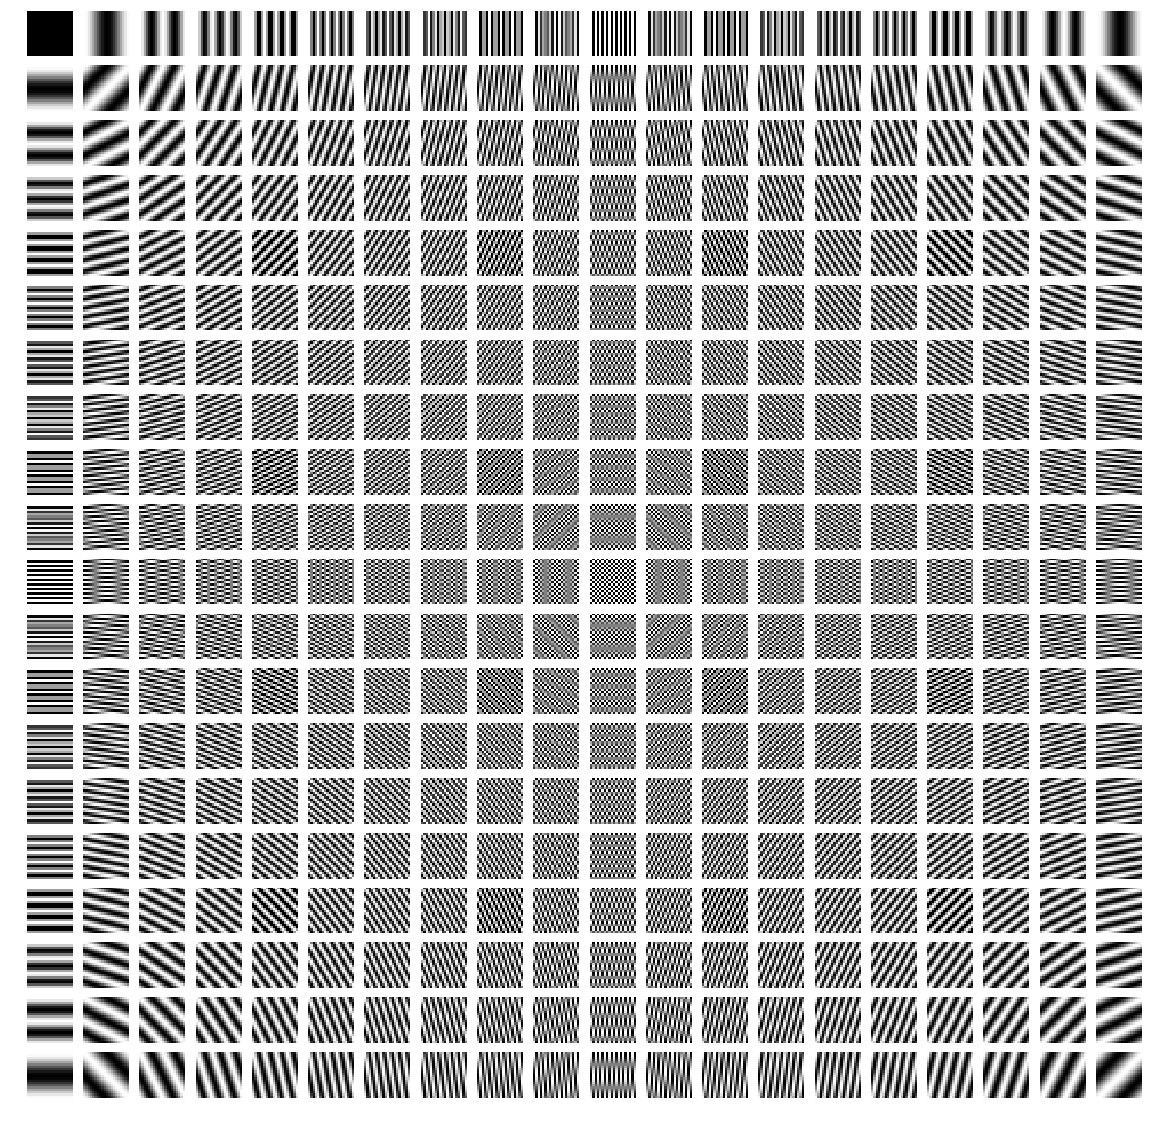
\includegraphics[scale=0.2]{images/fourier_basis.jpg}
        \end{tabular}
    \end{table}
\end{center}

Слева изображен базис в нумерации, используемой выше. Базисные элементы с большими или маленькими $k, l$ называются низкочастотными (потому, что каждый элемент базиса -- это переодические полоски, и чем экстремальнее значения индексов, тем они реже), а со средними -- высокочастотными. Низкочастотные компоненты изображения (то есть слагаемые в разложении на базисные вектора) отвечают за общий вид изображения, а высокочастотные -- за мелкие детали. Теперь разберемся, зачем это может быть нужно.

Теперь разберемся, как можно применить преобразование Фурье.

\subsection*{Быстрые свертки.}
    Сверткой изображения $X \in \mathbb{C}^{N \times M}$ с ядром $Y \in \mathbb{C}^{K \times L}$ называется изображение $Z \in \mathbb{C}^{N + K - 1 \times M + L - 1}$:
    \begin{gather*}
        Z[x, y] = \sum\limits_{s = \max(0, x - N + 1)}^{\min(K, x)}\sum\limits_{t = \max(0, y - M + 1)}^{\min(L, y)} Y[s, y] \cdot X[x - s, y - t]
    \end{gather*}
    
    Обозначение: $Z = (X \ast Y)$
    
    Свертки часто используются в анализе и обработке изображений, однако наивное вычисление занимает $\mathcal{O}(NMKL)$ времени, что много для больших размеров ядер.
    
    Однако на помощь приходит \textit{Теорема о свертке}:
    
    \begin{gather*}
        \hat{F}(X \ast Y) = \hat{F}(X') \hat{F}(Y')
    \end{gather*}
    
    Где $X', Y'$ -- это $X, Y$ добитые нулями справа и снизу до $(N + K - 1, M + L - 1)$.
    
    То есть, чтобы посчитать свертку двух изображений, надо:
    \begin{itemize}
        \item Добить их нулями до нужного размера
        \item Посчитать преобразование Фурье от каждого из них
        \item Поэлементно перемножить
        \item Взять обратное преобразование
    \end{itemize}
    
    Осталось заметить, что прямое и обратное преобразование Фурье можно вычислить за $\mathcal{O}(NM \log(NM))$ времени. [Немного деталей: чтобы это сделать, достаточно уметь \href{https://ru.wikipedia.org/wiki/Быстрое_преобразование_Фурье}{Быстро считать одномерные прямое и обратное преобразование фурье} и осознать, что двумерное преобразование -- это то же самое, что взять одномерное преобразование сначала независимо по столбцам, а потом по строкам]

\section*{Бесшовная склейка изображений}

\textbf{Задача}. Даны два изображения $X, Y$ (одинаковых размеров) и маска $M$ (массив того же размера из нулей и единиц). Единица означать, что надо брать пиксель из первого изображения, а нолик -- что из второго. Нужно создать коллаж.

\begin{center}
    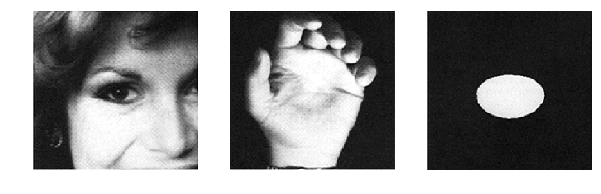
\includegraphics[scale=0.4]{images/task.png}
\end{center}

Если мы напрямую будем брать пиксели согласно маске, то переход между изображениями будет слишком резкий, а хочется его сгладить. 

\begin{center}
    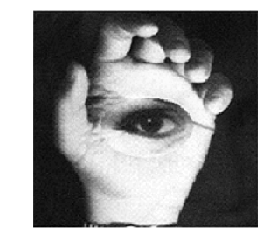
\includegraphics[scale=0.4]{images/naive.png}
\end{center}

Введем два понятия:

\begin{defn*} \textit{Гауссовской пирамидой} будем называть последовательность изображений, $G_0, G_1, \ldots, G_k$ полученных из исходного изображения $I_0$ сверткой с гауссовским фильтром:
\begin{gather*}
    G_0 = I_0 \\
    G_1 = G_0 \ast G \\
    \cdots \\
    G_k = G_{k - 1} \ast G
\end{gather*}

\textit{Лапласовской пирамидой} будем называть последовательность изображений, $L_0, L_1, \ldots, L_k$ полученных из гауссовской пирамиды операцией попарной разности
\begin{gather*}
    L_0 = G_0 - G_1 \\
    L_1 = G_1 - G_2 \\
    \cdots \\
    L_{k - 1} = G_{k - 1} - G_k
    L_k = G_k
\end{gather*}
\end{defn*}

Замечание: обычно в определение гауссовской пирамиды добавляют еще и операцию уменьшения размера изображения в два раза после применения свертки (отсюда и название -- пирамида), то есть $G_i = Subsample(G_{i - 1} \ast G)$. В определении палдасовской пирамиды, соответственно, 
$L_i~=~G_i~-~Upsample(G_{i + 1})$, но в нашем случае это нужно разве что для ускорения вычислений.

Итак, давайте посмотрим, что же происходит с точки зрения частот в этих пирамидах. Для этого надо заметить, что фурье-образ гауссовского фильтра -- гауссовский фильтр.

Тогда в $G_0$ у нас есть все изображение, а дальше мы начинаем последовательно убирать высокие частоты, оставляя только низкие.


\begin{center}
    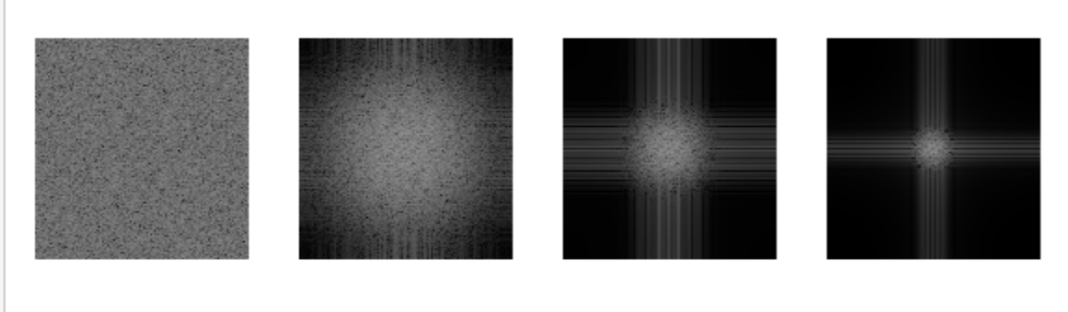
\includegraphics[scale=0.4]{images/G.png} 

    (изображены абсолютные значения преобразования Фурье, где ближе к центру изображены коэффициенты, отвечающие более низким частотам)
\end{center}


Что же происходит в лапласовской пирамиде? Для этого осознаем, что преобразование Фурье -- линейная операция и вычитание в обычных координатах соответствует вычитанию в базисе Фурье. Если в $G_0$ у нас есть все частоты, а в $G_1$ -- только низкие, то в $L_0 = G_0 - G_1$ у нас останутся только высокие частоты. Аналогично, в $L_1 = G_2 - G_1$ мы получим некоторую среднюю полосу частот (более низких, чем в $L_0$). Аналогично, в $L_2$ мы получаем еще более низкую полосу частот и так далее, пока в $L_k$ не останутся только самые низкие частоты.

\begin{center}
    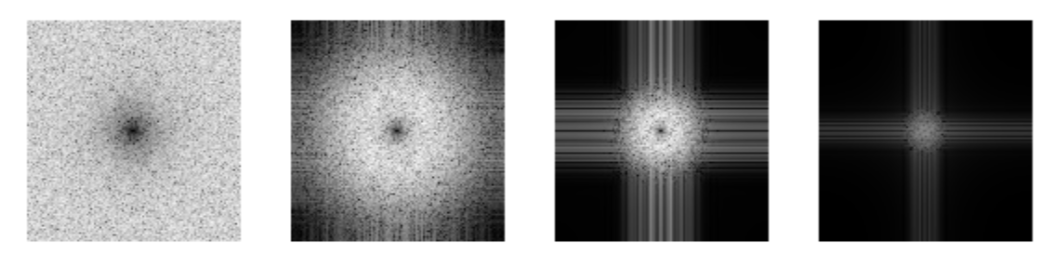
\includegraphics[scale=0.4]{images/L.png}
\end{center}

Заметим, что если сложить все элементы лапласовской пирамиды, то получится исходное изображение.

Идея алгоритма: поскольку мелкие детали изображений проявляются только в высоких частотах, их мы будем склеивать с помощью более резкой маски, а низкие частоты будем склеивать более плавной маской. Это и даст нам искомую плавность на границах.

Алгоритм:

\begin{enumerate}
    \item Вычисляем лапласовские пирамиды исходных изображений ${L}^X$ и ${L}^Y$, а так же гауссовскую пирамиду маски ${G}^M$
    \item Комбинируем поуровнево лапласовские пирамиды с помощью пирамиды масок:
    \begin{gather*}
        L_i = L^X_i \cdot G^M_i + (1 - G^M_i) \cdot L^Y_i
    \end{gather*}
    \item Получаем результат суммируя получившуюся пирамиду 
    \begin{gather*}
        C = \sum\limits_i L_i
    \end{gather*}
\end{enumerate}

Пример:

\begin{center}
    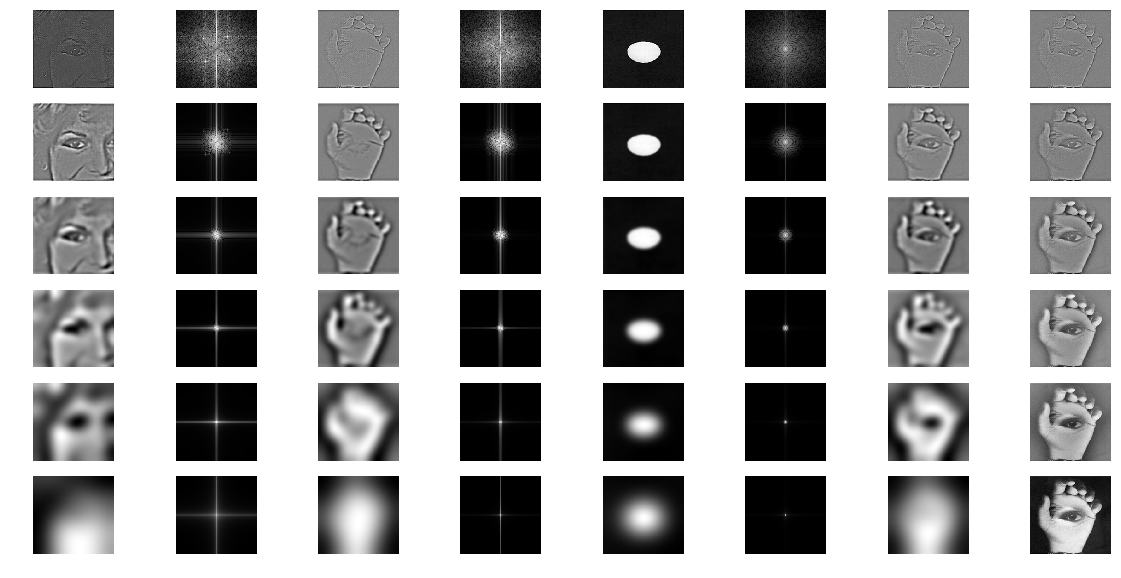
\includegraphics[scale=0.4]{images/example.png}
    
    (Изображены: $L^X, \hat{F}(L^X), L^Y, \hat{F}(L^Y), G^M, \hat{F}(G^M), L_i, \sum\limits_{k = 0}^i L_i$)
\end{center}

Заметим, что преобразованием Фурье мы пользовались лишь в теоретических рассуждениях, на практике мы его не вычисляли.

\section*{JPEG}

Разберемся, как работает алгоритм сжатия JPEG. 

\begin{enumerate}
    \item Для начала изображение переводится в другое цветовое пространство так, чтобы одним из каналов стала яркость. В случае JPEG это YCbCr:
    
    \begin{align*}
        Y'&=&0&+(0.299&\cdot R'_{D})&+(0.587&\cdot G'_{D})&+(0.114&\cdot B'_{D})\\
        C_{B}&=&128&-(0.168736&\cdot R'_{D})&-(0.331264&\cdot G'_{D})&+(0.5&\cdot B'_{D})\\
        C_{R}&=&128&+(0.5&\cdot R'_{D})&-(0.418688&\cdot G'_{D})&-(0.081312&\cdot B'_{D})
    \end{align*}
    
    Далее компоненты $C_B$ и $C_R$ уменьшаются в два раза, потому что, с одной стороны, это позволяет сэкономить метсто, а с другой -- не сильно меняет визуальное восприятие (после разжатия), так как человеческий глаз более восприимчив к $Y$ компоненте, нежели к цветным.
    
    После этого каждый из каналов разбивается на блоки $8\times8$ и каждый блок обрабатывается отдельно.
    
    \item Из каждого блока вычитается 128 (если раньше значения были от 0 до 255, то теперь они от -128 до 128)
    
    \item Далее к блоку применяется дискретное косинусное преобразование (DCT) -- это как дискретное преобразование Фурье, только мы раскладываем изображение не по базису комплексных экспонент, а по базису $E_{k, l}[n, m] \propto  \cos \frac{\pi (2n + 1)k}{2N}\cos\frac{\pi (2m + 1)l}{2M}$:
    
    \begin{center}
        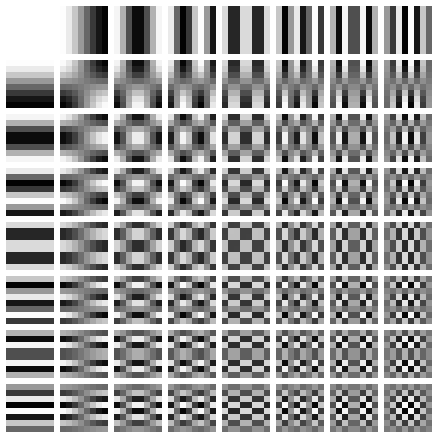
\includegraphics[scale=0.4]{images/DCT-8x8.png}
    \end{center}
    
    \item Далее происходит квантование амплитуд -- мы нацело поэлементно делим результат DCT на специальную матрицу -- матрицу квантования (зависящую от заранее выбраного параметра качества).
    
    Пример матрицы для качества в 50\%:
    \begin{gather*}
        Q={\begin{bmatrix}16&11&10&16&24&40&51&61\\12&12&14&19&26&58&60&55\\14&13&16&24&40&57&69&56\\14&17&22&29&51&87&80&62\\18&22&37&56&68&109&103&77\\24&35&55&64&81&104&113&92\\49&64&78&87&103&121&120&101\\72&92&95&98&112&100&103&99\end{bmatrix}}    
    \end{gather*}
    
    Смысл в том, что человеческий глаз получает большую часть информации из низких частот изображения, поэтому потерять информацию о высоких частотах не так страшно. Поэтому в матрице квантования более высоким частотам соответствуют более высокие значения -- чтобы после деления нацело получить ноль с высокой вероятностью.
    
    \item После этого у нас получается матрица с большим количеством нулей. Мы ее обходим (зигзагом), после чего применяем \href{https://ru.wikipedia.org/wiki/Кодирование_длин_серий}{кодирование длин серий}, а затем \href{https://ru.wikipedia.org/wiki/Код_Хаффмана}{кодирование Хаффмана}
    
Чтобы раскодировать JPEG надо применить все в обратном порядке -- для каждого блока раскодировать код Хаффмана и код серий, умножить на матрицу квантования, применить обратное дискретное косинусное преобразование, прибавить 128. Далее соединить все блоки в нужном порядке, увеличить размеры цветовых компонент и перевести обратно в RGB пространство.
    
\end{enumerate}

\section*{Список источников}

\begin{itemize}
    \item Курс ШАДа "Анализ изображений и видео (часть 1)". В открытом доступе отсутствует, но эти темы освещены в курсе \href{https://stepik.org/course/1280}{того же семинариста на stepik.org}
    \item \href{https://en.wikipedia.org/wiki/JPEG}{Wikipedia: JPEG}
    \item \href{https://docs.scipy.org/doc/}{Scipy documentation}
\end{itemize}

\end{document}


 